\newpage


\pagestyle{fancy}
\fancyhf{} 
\fancyhead[L]{{\footnotesize \textbf{\shortprojname}}\hfill{\footnotesize \leftmark}}
\fancyfoot[C]{\thepage}


\chapter{PROJECT DESCRIPTION} \label{chap:ProjDesc}

\section{\fontsize{14}{16} Working Principle}
{
	\fontsize{12}{14}
	The RAVEN’s working principle is a combination of particulate processes which involves:
	
	\begin{itemize}
		\item \textbf{Data Acquisition:} The UGV improves situational awareness by using depth cameras
		and LiDAR to collect environmental data, ensuring precise navigation and effective
		obstacle detection through continuous sensor data acquisition.
		
		\item \textbf{Data Transmission:} Utilize the DDS provided by ROS2 for reliable and efficient data
		sharing, while establishing strong wireless connections to enable remote control and
		real-time tracking.
		
		\item \textbf{Localization:} Integrate depth camera and LiDAR data to enhance the robot's
		perception of its surroundings, and employ SLAM to create dynamic maps and localize
		the robot within them.
		
		\item \textbf{Data Storage:} While navigating, temporarily store data for quick processing, and keep
		sensor data and maps for future use and analysis.
		
		\item \textbf{Analysis and Visualization:} Utilize programs like rViz2 to visualize the robot's current
		state, surroundings, and mapping progress, while analyzing sensor data to identify and
		classify obstacles for informed navigation.
		
		\item \textbf{Path Planning:} Use Nav2 for dynamic path planning, enabling real-time navigation
		around obstacles, and implementing decision-making algorithms to adapt to complex
		environments and meet operational goals.
		
		\item \textbf{Feedback and Control:}  Implement feedback systems to refine navigation for seamless
		operation, utilizing real-time sensor data to prevent collisions with both static and
		dynamic obstacles.
		
		\item \textbf{User Interaction:} Provide operators with a user interface to monitor environmental
		data and the robot's status, while allowing manual control when necessary to enhance
		flexibility and manage challenging tasks.
		
		\item \textbf{Safety Mechanisms:} Implement immediate stop features for safety in the event of
		detected anomalies, and use real-time sensor data to proactively avoid collisions during
		navigation.
	\end{itemize}
	
	To function, the UGV gathers real-time data from depth and LiDAR cameras, which are then
	relayed and analyzed to provide quick insights. GPS and odometry improve localization, and
	SLAM creates dynamic maps. Effective path planning is supported by NAV2, and real-time
	modifications are possible thanks to feedback systems. Through emergency procedures and
	power management, user features provide safety while enabling manual control and
	monitoring.
	

}

% Subsection for Block Diagram
\subsection{Block Diagrams}

% Subsubsection for System Block Diagram
\subsubsection{System}
	\begin{figure}[H]
		\centering
		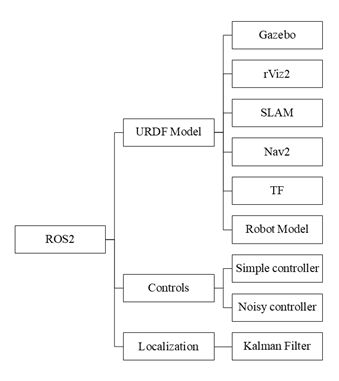
\includegraphics{images/Content/system_block_dia.png}
		\caption{ROS2 system block diagram}
		\label{fig:fig1}
	\end{figure}

% Subsubsection for URDF Block Diagram
\subsubsection{URDF}
	\begin{figure}[H]
		\centering
		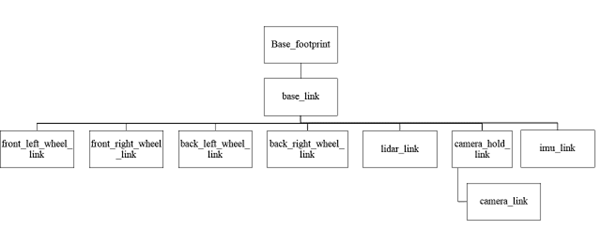
\includegraphics[scale=0.9]{images/Content/URDF_block_dia.png}
		\caption{URDF system block diagram}
		\label{fig:fig2}
	\end{figure}


\subsection{\fontsize{14}{16} Flow Chart}
	\begin{figure}[H]
		\centering
		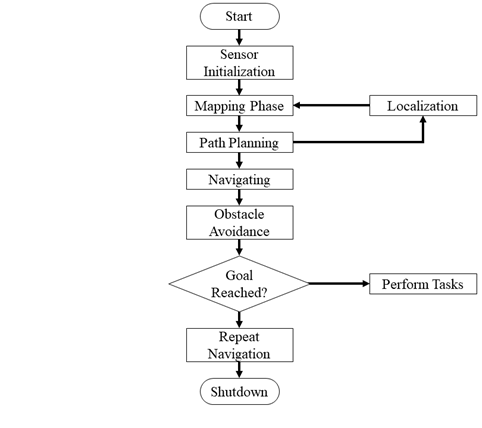
\includegraphics{images/Content/flow_chart.png}
		\caption{Flow chart representation}
		\label{fig:fig3}
	\end{figure}

\section{\fontsize{14}{16} Software Requirements}
{
	\fontsize{12}{14}
	Simulating a Jetson-based robot involves the integration of various software components and
	frameworks that facilitate the development, testing, and deployment of the robotics application.
	A list of the key software required are:
	
	\begin{itemize}
		\item NVIDIA JetPack SDK
		
		\item ROS2 Humble Hawksbill
		
		\item rViz2
		
		\item Joint State Publisher
		
		\item Gazebo
		
		\item PlotJuggler
		
		\item SLAM
		
		\item Nav2
		
		\item CMake
		
		\item VS Code
	\end{itemize}
		
}

\section{\fontsize{14}{16} Software Design}
{
	\fontsize{12}{14}
	The integration of URDF, RViz2, and Gazebo provides a comprehensive framework for
	designing, visualizing, and simulating robotic system.
	
	\begin{enumerate}[label=\textbf{\arabic*}.]
		\item \textbf{URDF structure} \par It provides a clear and concise way to describe the various components of a robot, including its
		links and joints.
				
		\begin{itemize}
			\item \textbf{Links:}
			\begin{itemize}
				\item Each link represents a rigid body in the robot.
		
				\item Links can have properties such as:
				\begin{itemize}
					\item \textbf{Inertial properties:} Mass, center of mass, and inertia matrix.
					\item \textbf{Visual properties:} Geometry (shapes like boxes, spheres, and meshes), colors,
					and textures.
					\item \textbf{Collision properties:} Shapes used for collision detection.
				\end{itemize}
			\end{itemize}
			\item \textbf{Joints:}
			\begin{itemize}
				\item Joints define the relationship between two links and the type of movement allowed.
				\item Types of joints include:
				\begin{itemize}
					\item \textbf{Revolute:} A hinge joint that rotates around an axis with specified upper and
					lower limits.
					\item \textbf{Continuous:} A hinge joint that rotates around an axis without limits.
					\item \textbf{Prismatic:} A sliding joint that moves along an axis with specified upper and
					lower limits.
					\item \textbf{Fixed:} A non-moving joint that locks all degrees of freedom, requiring no
					additional specifications.
					\item \textbf{Floating:} A joint that allows motion in all six degrees of freedom.
					\item \textbf{Planar:} A joint that permits movement within a plane perpendicular to the axis.
				\end{itemize}
				\item Each joint should specify:
				\begin{itemize}
					\item \textbf{Parent and child links:} Which links the joint connects.
					\item \textbf{Axis of movement:} Direction in which the joint can move.
					\item \textbf{Limits:} Maximum and minimum positions for joints that allow movement.
				\end{itemize}
			\end{itemize}
		\end{itemize}

	\captionsetup[subfloat]{font={normalsize}}
		
	\begin{figure}[H]
		\centering
		\subfloat[Links Element]{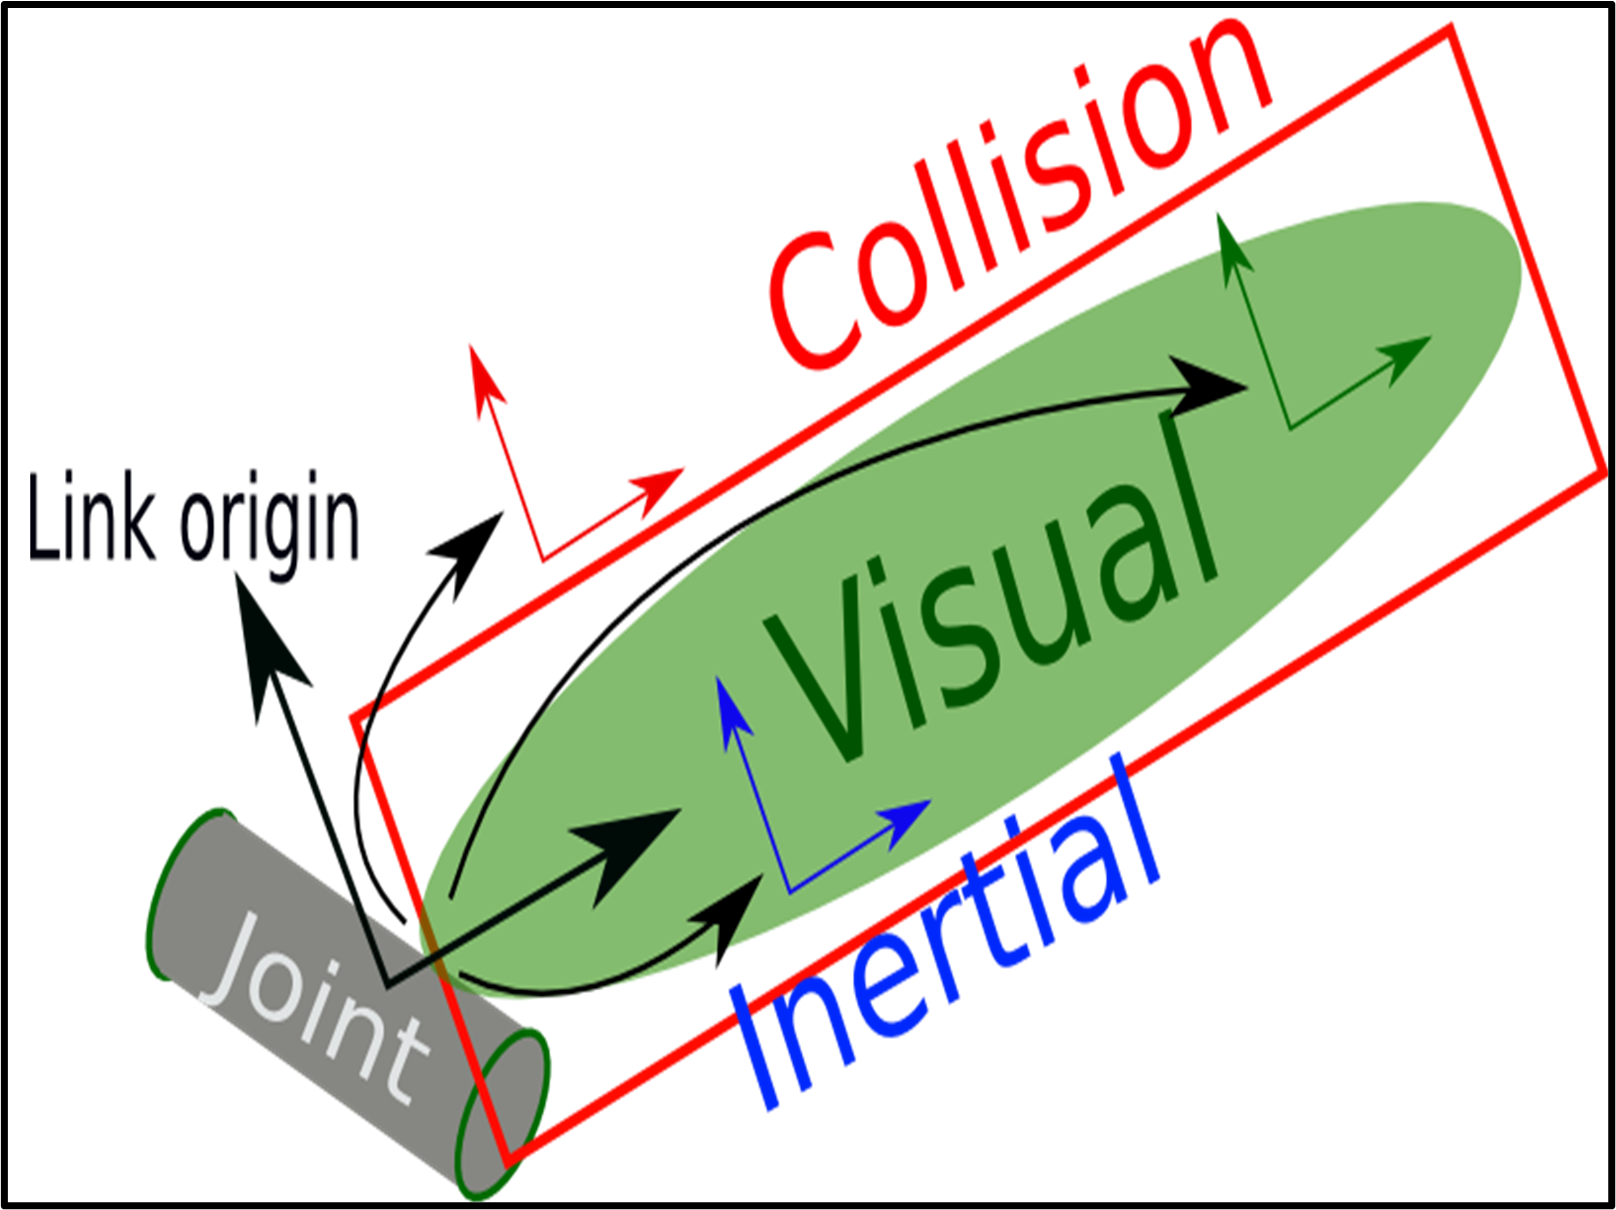
\includegraphics[width=0.45\textwidth]{images/Content/links_elem.png}} 
		\hfill
		\subfloat[Joints Element]{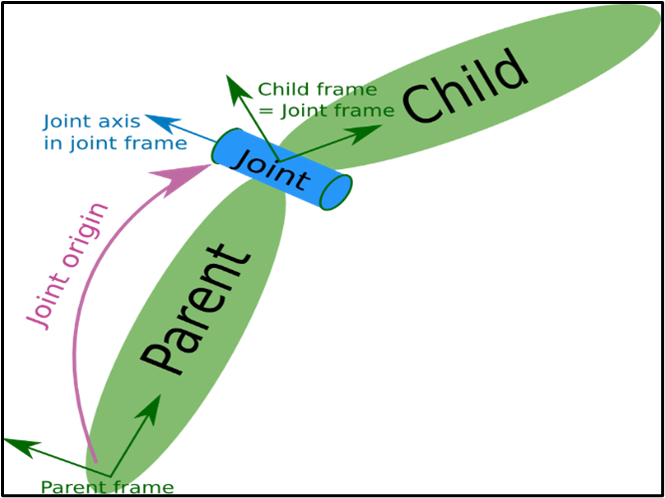
\includegraphics[width=0.45\textwidth]{images/Content/joints_elem.png}} 
		\hfill
		\caption{Links and Joints \cite{links} \cite{joints}} 
		\label{fig:fig4}
	\end{figure}
	
	
	
	
		\item \textbf{RViz2 visualization of the movement of links} \par The RViz2 configuration include:
		\begin{itemize}
			\item Loading the URDF model to visualize the robot structure.
			\item Setting up appropriate displays for joint states and sensor data.
			\item Configuring the frame of reference for accurate visualization.
		\end{itemize}
		
		\item \textbf{Gazebo (Simulation and Navigation)}
		\begin{itemize}
			\item \textbf{SLAM (Simultaneous Localization and Mapping)} \par Gazebo is a robust simulation environment that allows for realistic robot modeling and testing. It integrates with ROS for powerful simulation features, including SLAM capabilities.
			\begin{itemize}
				\item Supports various SLAM algorithms for mapping and localization.
				\item Uses sensor data (e.g., LiDAR, camera) to create a map of the environment while
				keeping track of the robot's position within that map.
			\end{itemize}
			
			\item \textbf{Nav2 (Navigation Stack)} \par Nav2 is the navigation framework for ROS 2, enabling autonomous navigation for
			mobile robots. It includes several components for path planning, obstacle avoidance, and goal reaching.
			\begin{itemize}
				\item \textbf{Global Planner:} Calculates an optimal path from the robot's current position to the desired goal.
				\item \textbf{Local Planner:} Adjusts the robot's path in real-time, considering dynamic obstacles and the robot's kinematics.
				\item \textbf{Costmaps:} Maintains a representation of the environment, including static and dynamic obstacles, to inform the planning process.
			\end{itemize}
		\end{itemize}
	\end{enumerate}
}

\section{\fontsize{14}{16} Software Description}
\subsection{\fontsize{14}{16} NVIDIA JetPack SDK}
{
	\fontsize{12}{14}
	The NVIDIA JetPack SDK is an essential software development kit for NVIDIA Jetson devices, providing the necessary tools and libraries to develop AI-based applications. Below
	are the specifications and key components of the JetPack SDK:
	\begin{itemize}
		\item \textbf{CUDA Toolkit:} Parallel computing platform and API model for GPU computing.
		\item \textbf{cuDNN:} GPU-accelerated library for deep neural networks, optimizing performance for training and inference.
		\item \textbf{TensorRT:} High-performance deep learning inference optimizer and runtime, enabling fast deployment of AI models.
		\item \textbf{VisionWorks:} A development package for computer vision applications, providing GPU-accelerated image processing.
		\item \textbf{OpenCV:} Library of programming functions for real-time computer vision, included in the JetPack SDK.
		\item \textbf{L4T:} An operating system that includes the necessary drivers and libraries for Jetson hardware.
	\end{itemize}
	
	\begin{figure}[H]
		\centering
		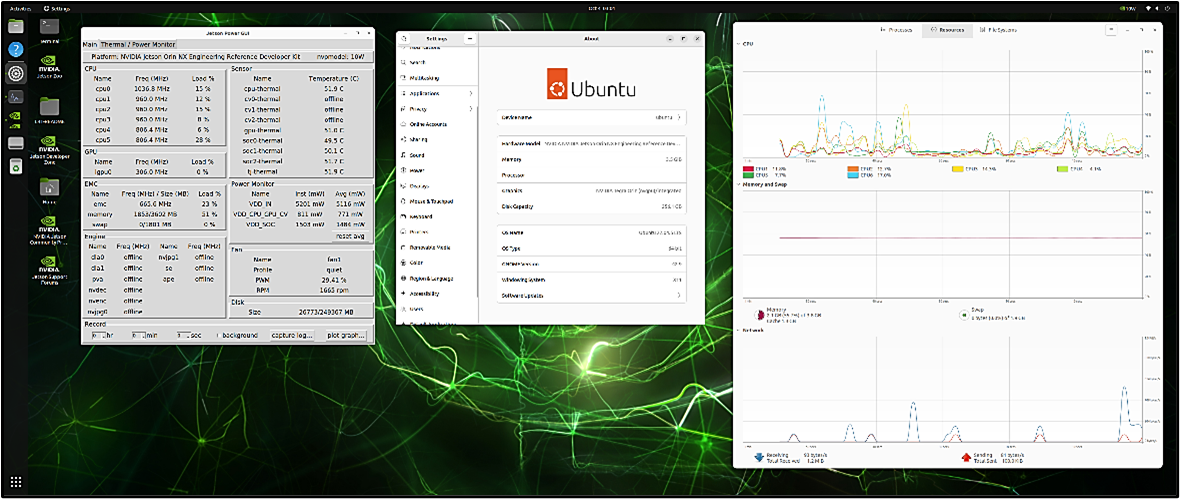
\includegraphics{images/Content/Ubuntu}
		\caption{Ubuntu 22.04 with NVIDIA JetPack SDK}
		\label{fig:ubuntu}
	\end{figure}
}

\subsection{\fontsize{14}{16} ROS2 Humble Hawksbill}
{
	\fontsize{12}{14}
	ROS 2 Humble Hawksbill is the eighth release of ROS 2 and is notable for several key features and improvements. Below is an overview of its specifications and highlights:
	\begin{itemize}
		\item \textbf{LTS:} Supported until May 2027.
		\item \textbf{Ubuntu Compatibility:} Officially supports Ubuntu 22.04 (Jammy Jellyfish).
		\item \textbf{Enhanced Performance:} Improvements in real-time capabilities and inter-process 		communication.
		\item \textbf{New Packages:} Updates in navigation, perception, and robot control.
		\item \textbf{Documentation \& Community:} Robust resources and support available.
	\end{itemize}
	
	\begin{figure}[H]
		\centering
		
\includegraphics{images/Content/ros2_humble}
		\caption{ROS2 Humble \cite{ros2_humble}}
		\label{fig:ros2humble}
	\end{figure}
}

\subsection{\fontsize{14}{16} rViz2}
{
	\fontsize{12}{14}
	rViz2 is a powerful visualization tool designed for ROS 2. It allows users to visualize various
	types of data related to their robotic systems, making it easier to understand and debug complex
	interactions. Below are the key specifications and features of rViz2:
	\begin{itemize}
		\item \textbf{Graphical Interface:} Provides a user-friendly graphical interface to visualize robot
		models, sensor data, maps, and more.
		\item \textbf{Plugin Architecture:} Supports a wide range of plugins, enabling users to visualize
		different types of data and customize their workspace according to their needs.
		\item \textbf{3D Visualization:} Offers 3D visualization capabilities, allowing users to see their robot
		and environment more intuitively.
		\item \textbf{Frame Transformation:} The frame transformation library is pluggable, meaning users
		can load and change different transformation library plugins as needed.
		\item \textbf{Data Display:} Capable of displaying various data types, including point clouds,
		images, and robot states, which helps in monitoring and debugging.
	\end{itemize}
	
	\begin{figure}[H]
		\centering
		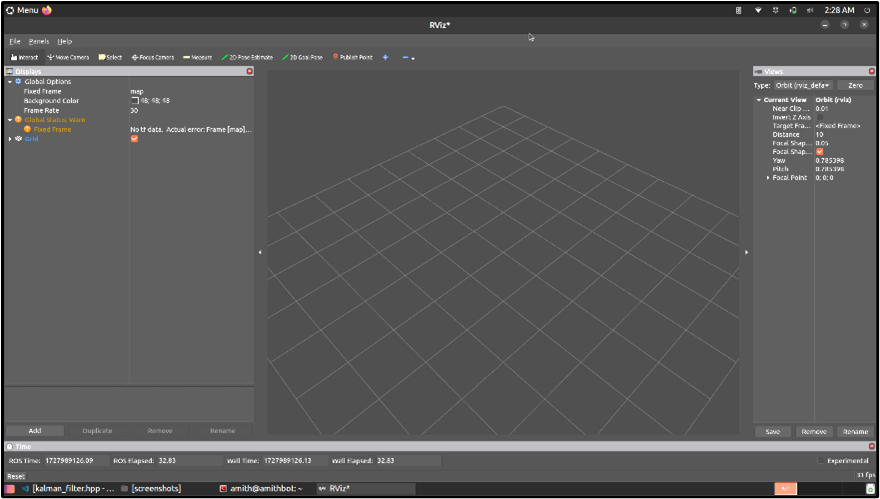
\includegraphics{images/Content/rviz2}
		\caption{rViz2}
		\label{fig:rviz2}
	\end{figure}
}

\subsection{\fontsize{14}{16} Joint State Publisher}
{
	\fontsize{12}{14}
	Joint State Publisher is a ROS 2 package that allows users to publish the state of a robot's joints.
	This tool is particularly useful in robotic applications for simulating and visualizing joint states.
	Below are the key specifications and features of the Joint State Publisher:
	\begin{itemize}
		\item \textbf{Joint State Publishing:} Publishes the state of all joints in a robot model, allowing for
		real-time monitoring and control.
		\item \textbf{GUI:} Includes a simple GUI that enables users to manually adjust the positions of the
		joints, facilitating interactive testing and visualization.
		\item \textbf{Integration with URDF:} Works seamlessly with URDF models, making it easy to
		visualize joint states based on the robot's configuration.
	\end{itemize}
	
	\begin{figure}[H]
		\centering
		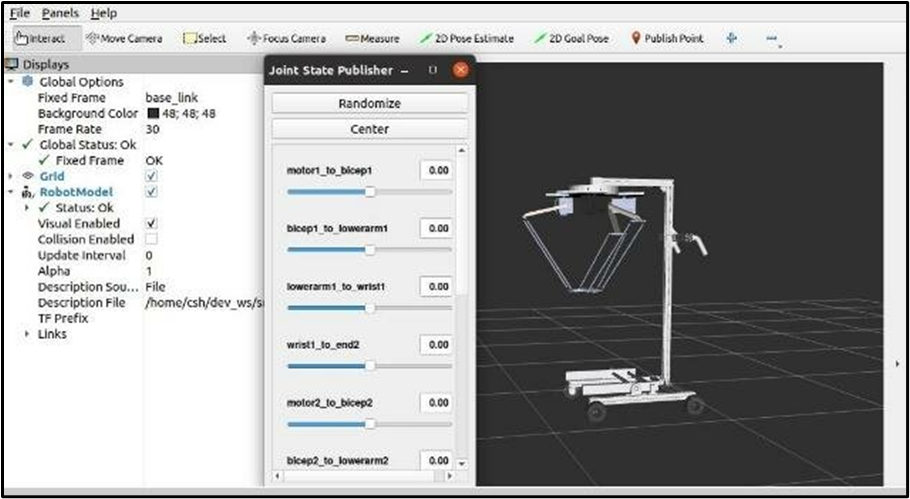
\includegraphics{images/Content/jspgui}
		\caption{Joint State Publisher GUI \cite{jointstatepub}} 
		\label{fig:jspgui}
	\end{figure}
}

\subsection{\fontsize{14}{16} Gazebo}
{
	\fontsize{12}{14}
	Gazebo is a powerful simulation tool designed for testing robot models in complex environments. It provides advanced physics simulation, rendering capabilities, and a user- friendly interface. Below are the key specifications and features of Gazebo:
	\begin{itemize}
		\item \textbf{3D Simulation:} Offers high-fidelity 3D simulation of robots and their environments,
		allowing users to visualize interactions in real-time.
		\item \textbf{Physics Engines:} Supports multiple physics engines enabling accurate modeling of
		physical interactions such as collisions and gravity.
		\item \textbf{Sensor Simulation:} Simulates a variety of sensors including cameras, LIDAR, and
		IMUs, allowing for realistic testing of robotic perception and navigation.
		\item \textbf{Integration with ROS:} Fully compatible with ROS and ROS 2, facilitating easy
		integration of robotic algorithms with simulated environments.
		\item \textbf{World Building:} Provides tools for creating and editing complex environments with
		customizable terrains, obstacles, and lighting.
	\end{itemize}
	
	\begin{figure}[H]
		\centering
		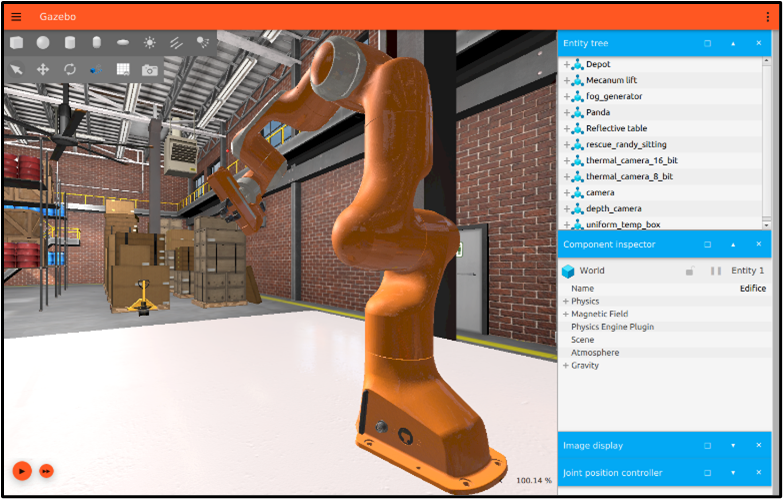
\includegraphics{images/Content/gazebo}
		\caption{Gazebo interface \cite{gazebo_github}}
		\label{fig:gazebo}
	\end{figure}
}

\subsection{\fontsize{14}{16} PlotJuggler}
{
	\fontsize{12}{14}
	PlotJuggler is a versatile tool designed for visualizing time-series data, particularly in robotics
	and simulation contexts. It allows users to plot, analyze, and interact with data streams in real
	time. Below are the key specifications and features of PlotJuggler:
	\begin{itemize}
		\item \textbf{Real-Time Data Visualization:} Supports real-time plotting of time-series data, making
		it ideal for monitoring robot states, sensor outputs, and other dynamic data.
		\item \textbf{Flexible Data Import:} Capable of importing data from various sources, including ROS
		topics, CSV files, and custom data streams.
		\item \textbf{Multi-Plot Capability:} Allows for multiple plots to be displayed simultaneously,
		enabling comparative analysis of different data streams.
	\end{itemize}
	
	\begin{figure}[H]
		\centering
		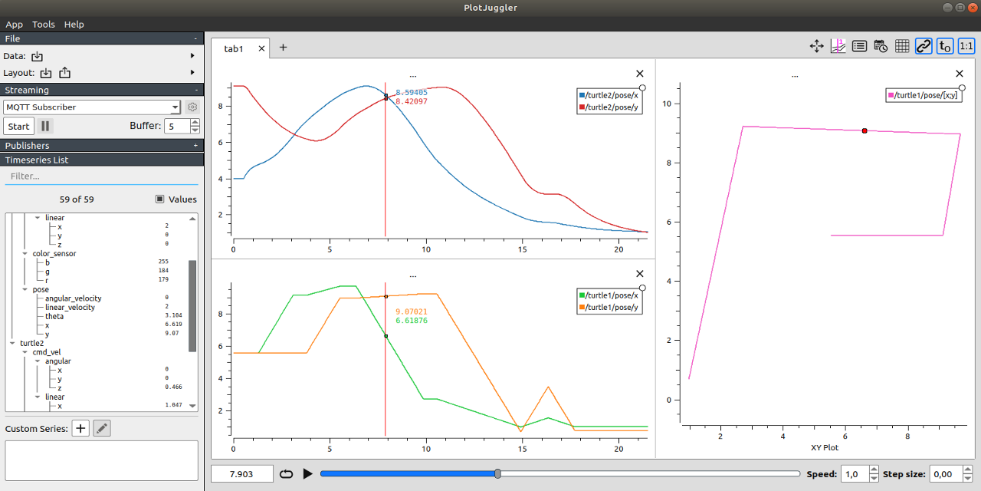
\includegraphics{images/Content/plotjug}
		\caption{PlotJuggler \cite{plotjuggler_github}}
		\label{fig:plotjug}
	\end{figure}
}

\subsection{\fontsize{14}{16} SLAM}
{
	\fontsize{12}{14}
	SLAM is a technology used in robotics and computer vision that allows a device to create a map of an unknown environment while simultaneously determining its location within that map. Here are the key specifications of SLAM systems:
	\begin{itemize}
		\item \textbf{Real-Time Processing:} Ability to process data and update maps in real-time, enabling
		immediate feedback and navigation.
		\item \textbf{Loop Closure Detection:} Recognizing previously visited locations to correct drift and
		improve map accuracy.
		\item \textbf{Data Association:} Matching measurements from sensors to features in the map to
		maintain consistency.
		\item \textbf{Scalability:} Effective performance in both small and large environments without
		significant loss of accuracy.
	\end{itemize}
}

\subsection{\fontsize{14}{16} Nav2}
{
	\fontsize{12}{14}
	Nav2 is a powerful navigation framework designed to enable mobile robots to navigate autonomously. Below are the key specifications and features of the Nav2 framework.
	\begin{itemize}
		\item \textbf{Global Planner:} Responsible for generating a global path from the robot's start position
		to the goal position and utilizes algorithms like A* or Dijkstra’s for pathfinding.
		\item \textbf{Local Planner:} Handles real-time adjustments to the path based on dynamic obstacles
		and changes in the environment and works closely with the robot's sensors to ensure
		safe navigation.
		\item \textbf{Lifecycle Management:} Each component of Nav2 can be managed through a lifecycle
		interface, allowing for better control over the state of the navigation stack.
		\item \textbf{Sensor Integration:} Supports various sensor inputs, including LIDAR, cameras, and
		IMUs, for effective navigation in diverse environments.
		\item \textbf{Dynamic Reconfiguration:} Parameters can be adjusted at runtime without stopping
		the navigation process.
		\item \textbf{Behavior Trees:} Uses behavior trees for managing high-level navigation tasks,
		providing a clear structure for managing complex behaviors.
	\end{itemize}
	
	\begin{figure}[H]
		\centering
		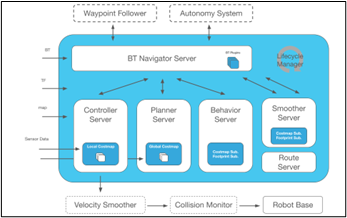
\includegraphics{images/Content/nav2arch}
		\caption{Nav2 architecture \cite{nav2_docs}}
		\label{fig:nav2arch}
	\end{figure}
}

\subsection{\fontsize{14}{16} CMake}
{
	\fontsize{12}{14}
	CMake is an open-source build system generator that uses a simple configuration file to manage the build process of software projects across different platforms. It is widely used in the C++ community for managing project dependencies and building applications. Below are the key features of CMake.
	\begin{itemize}
		\item \textbf{Cross-Platform Support:} CMake can generate build files for various platforms,
		including Windows, Linux, and macOS, allowing for consistent builds across different
		environments.
		\item \textbf{Build System Generation:} Supports multiple build systems, such as Makefiles, Ninja,
		Visual Studio, and Xcode, enabling developers to choose their preferred environment.
		\item \textbf{Dependency Management:} Facilitates the management of project dependencies,
		allowing for easy inclusion of external libraries and packages.
		\item \textbf{Modularization:} Supports the creation of modular projects with subdirectories and
		separate \emph{CMakeLists.txt} files for each module.
	\end{itemize}
}

\subsection{\fontsize{14}{16} VS Code}
{
	\fontsize{12}{14}
	VS Code is a popular, open-source code editor developed by Microsoft. It is designed to be lightweight yet powerful, providing developers with a variety of features to enhance productivity. Below are the key specifications and features of Visual Studio Code.
	\begin{itemize}
		\item \textbf{IntelliSense:} Provides intelligent code completion, parameter info, quick info, and
		member lists, enhancing coding efficiency.
		\item \textbf{Debugging:} Built-in debugging support for various programming languages, allowing
		developers to set breakpoints, inspect variables, and navigate through code.
		\item \textbf{Extensions and Customization:} A rich ecosystem of extensions available through the
		Visual Studio Code Marketplace to add functionality, including support for additional
		languages, themes, and tools.
		\item \textbf{Integrated Terminal:} Built-in terminal support that allows users to run command-line
		tools directly within the editor, streamlining the development workflow.
	\end{itemize}
	
	\begin{figure}[H]
		\centering
		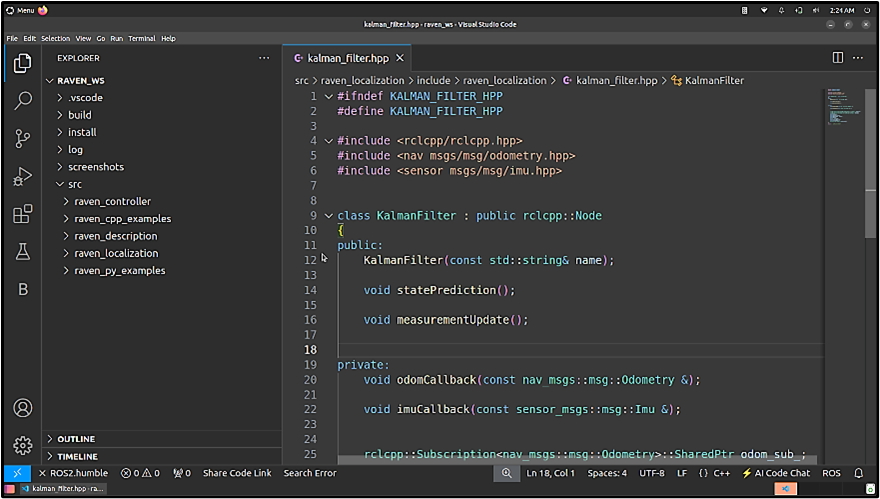
\includegraphics{images/Content/vscodeui}
		\caption{VS Code user interface}
		\label{fig:vscodeui}
	\end{figure}
}